\chapter{Finite element analysis in a nutshell}
In the previous chapters we learned to optimize discrete truss structures. However, most structures are not discrete by nature. They are continua and need to be transferred to a discrete representation for structural optimization. The most common method for this is the \emph{Finite Element Method} (FEM) and we quickly summarize this method in this chapter for further use in structural optimization. If you are interested in more details, you may refer to the excellent book by Fish and Belytschko \cite{Fish2007}.

\begin{objectives}{}{objectives_fem}
After studying this chapter and finishing the exercise, you should be able to 
\begin{itemize}[label=$\dots$]
    \item explain why we need finite elements in the first place 
    \item cite the linear elastic problem for an isotropic material
    \item formulate the weak form of the linear elastic problem and explain advantages of that formulation
    \item describe the concept of discretization by finite elements 
    \item formulate the shape functions and derivatives for a 2D quadrilateral linear element 
    \item transform the weak form into a linear system of equations using shape functions and numerical integration
    \item assemble the global FEM system and draw analogies to truss systems
\end{itemize}
\end{objectives}

\section{The linear elastic problem}
The fundamental equation to solve in static structural problems is the balance of linear momentum
\begin{equation}
    \nabla \cdot \mathbf{S}(\mathbf{x}) + \mathbf{b}(\mathbf{x})= \mathbf{0} 
    \quad 
    \mathbf{x} \in \Omega
    \label{eq:linear_momentum_balance}
\end{equation}
with the symmetric stress tensor $\mathbf{S}=\mathbf{S}^\top \in \mathcal{R}^{d \times d}$ and a prescribed body force field $\mathbf{b} \in \mathcal{R}^d$ describing a force per volume. The term \emph{static} means that we do not consider any time derivatives, i.e. we are searching for a stationary solution.  The domain $\Omega$ describes for example all points of a structural component and we use $\partial \Omega$ to denote the boundary of that domain. This equilibrium basically states that the divergence of stresses (inner forces) must balance the body force field in all points of a domain $\Omega$ to remain stationary. 

The stress tensor is related to the engineering strain tensor 
\begin{equation}
    \mathbf{E}(\mathbf{u}) = \frac{1}{2} \left(\nabla \mathbf{u} + \left(\nabla \mathbf{u}\right)^\top \right)
    \label{eq:strain}
\end{equation} 
via a linear elastic material model 
\begin{equation}
    \mathbf{S}(\mathbf{x})  = \mathbb{C}  : \mathbf{E}(\mathbf{u}) 
    \label{eq:linear_elasticity}
\end{equation}
with a stiffness tensor $\mathbb{C}  \in \mathcal{R}^{d \times d \times d \times d}$. Here, it is assumed that $\mathbb{C}$ does not depend on the position $\mathbf{x}$, i.e. the same material is used in the entire structure. In case of an isotropic material, i.e. a material that behaves direction-independent, we can write Equation \eqref{eq:linear_elasticity} as
\begin{equation}
    \mathbf{S}(\mathbf{x}) = \mathbb{C}_\textrm{iso}  : \mathbf{E}(\mathbf{u})  =  2 G \mathbf{E}(\mathbf{u})  + \Lambda \textrm{tr}(\mathbf{E}(\mathbf{u}) ) \mathbf{I},
    \label{eq:isotropic_material}
\end{equation}
with so-called the Lamé constants 
\begin{equation}
    G = \frac{E}{2(1+\nu)} > 0 
    \quad \text{and} \quad 
    \Lambda = \frac{E\nu}{(1+\nu)(1-2\nu)} > 0 .
\end{equation} 
These two constants, respectively the two constants Young's modulus $E$ and Poisson ratio $\nu$ uniquely describe a linear elastic material. 

\begin{figure}[!htpb]
    \centering
    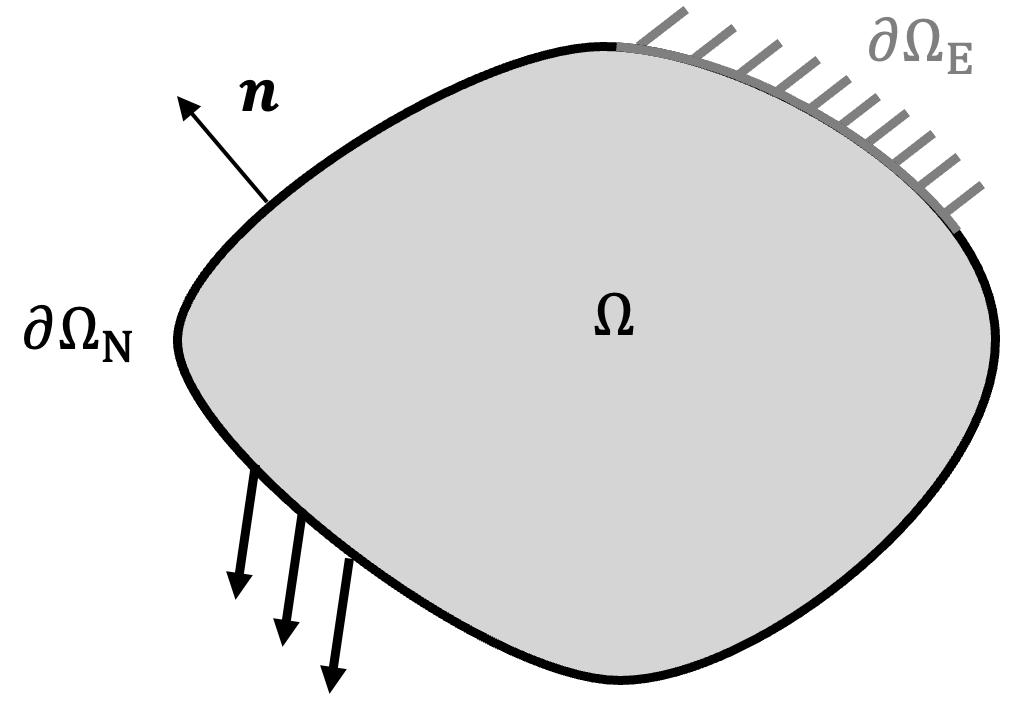
\includegraphics[width=0.5\textwidth]{figures/boundaries.png}
    \caption{The domain $\Omega$ has a boundary $\partial \Omega = \partial \Omega_E \cup \partial \Omega_N, \partial \Omega_E \cap \partial \Omega_N = \emptyset$. We prescribe a displacement $\mathbf{u}_0$ at the essential boundary $\partial \Omega_E$ illustrated with gray lines in the image. The remaining boundary $\partial \Omega_N$ is subjected to a surface traction $\mathbf{t}(\mathbf{x})$. The surface takes the form of a force per boundary unit, e.g. Newton per Meter in a two-dimensional problem with a one-dimensional boundary.}
    \label{fig:boundaries}
\end{figure}

% After substituting the constant isotropic linear elastic material model from Equation \eqref{eq:isotropic_material} in Equation \eqref{eq:linear_momentum_balance} we get Navier's equation
% \begin{equation}
%     (\Lambda + G) \nabla \cdot \left( \nabla \mathbf{u}(\mathbf{x}) 
% \right)
%     + G \nabla^2 \mathbf{u}(\mathbf{x})  + \mathbf{b}(\mathbf{x})  = \mathbf{0}.
%     \label{eq:navier}
% \end{equation}
% In this equation, displacements $\mathbf{u}(\mathbf{x})  \in \mathcal{R}^d$ are the only unknowns. 
% We may write Equation \eqref{eq:navier} more explicitly for the three-dimensional case by expanding it to
% \begin{align}
%     \label{eq:momentum_balance_mat_1}
%     (\Lambda + G) \left( \frac{\partial^2 u_1}{\partial x_1^2} + \frac{\partial^2 u_2}{\partial x_1 \partial x_2} + \frac{\partial^2 u_3}{\partial x_1 \partial x_3}\right)
%     + G \left( \frac{\partial^2 u_1}{\partial x_1^2} + 
%         \frac{\partial^2 u_1}{\partial x_2^2} + \frac{\partial^2 u_1}{\partial x_3^2} 
%     \right) + b_1 &= 0 \\
%     \label{eq:momentum_balance_mat_2}
%     (\Lambda + G) \left( \frac{\partial^2 u_1}{\partial x_1 \partial x_2} + \frac{\partial^2 u_2}{\partial x_2^2} + \frac{\partial^2 u_3}{\partial x_2 \partial x_3}\right)
%     + G \left( \frac{\partial^2 u_2}{\partial x_1^2} + 
%         \frac{\partial^2 u_2}{\partial x_2^2} + \frac{\partial^2 u_2}{\partial x_3^2} 
%     \right) + b_2 &= 0 \\
%     \label{eq:momentum_balance_mat_3}
%     (\Lambda + G) \left( \frac{\partial^2 u_1}{\partial x_1 \partial x_3} + \frac{\partial^2 u_2}{\partial x_2 \partial x_3} + \frac{\partial^2 u_3}{\partial x_3^2}\right)
%     + G \left( \frac{\partial^2 u_2}{\partial x_1^2} + 
%         \frac{\partial^2 u_2}{\partial x_2^2} + \frac{\partial^2 u_2}{\partial x_3^2} 
%     \right) + b_3 &= 0 
% \end{align}
% and observe that we have three partial differential equations for three unknowns $u_1(\mathbf{x}), u_2(\mathbf{x}), u_3(\mathbf{x})$.
With essential boundary conditions on $\partial \Omega_E$ and natural boundary conditions on $\partial \Omega_N$ (see Figure \ref{fig:boundaries}) we can formulate the boundary value problem of linear elasticity as 
\begin{align}
    \nabla \cdot \mathbf{S}(\mathbf{x}) + \mathbf{b}(\mathbf{x}) &= \mathbf{0} 
        &\mathbf{x} \in \Omega \\
    \mathbf{u}(\mathbf{x}) 
    &= \mathbf{u}_0 (\mathbf{x}) 
        &\mathbf{x} \in \partial \Omega_E \\
    \mathbf{S}(\mathbf{x}) \cdot \mathbf{n}(\mathbf{x}) 
    &= \mathbf{t} (\mathbf{x}) 
        &\mathbf{x} \in \partial \Omega_N\\
    \textrm{s.t.} \quad \mathbf{S} &= \mathbb{C} : \mathbf{E}(\mathbf{u})
\end{align}
 which should be solved for displacements $\mathbf{u}(\mathbf{x})$. This is a problem with three partial differential equations for three unknowns $u_1(\mathbf{x}), u_2(\mathbf{x}), u_3(\mathbf{x})$.
Note that this is a second order problem, as we have to compute second derivatives of $\mathbf{u}$ in this problem, as it is differentiated once by $\mathbf{E}(\mathbf{u})$ and then once by $\nabla \cdot \mathbf{S}(\mathbf{x})$.

% \begin{example}{Plane stress}{planestressexample} 
%     We may reduce the elastic problem to two dimensions, if we make an assumption about the third dimension. If we analyze a structure that is very thin in the 3-direction, e.g. a plate or membrane, there are no out-of-plane stress components and we may assume \emph{plane stress}, i.e. $S_{13}=S_{23}=S_{33}=0$ and $\frac{\partial S_{11}}{\partial x_3}=\frac{\partial S_{12} }{\partial x_3}=\frac{\partial S_{22}}{\partial x_3}=0$. 
    
%     Consider a two-dimensional rectangle $\Omega = [0,l]^2$ which is subjected to the following essential boundary conditions
%     \begin{equation}
%         u_1(0, x_2) = 0     \quad
%         u_1(l, x_2) = u_0   \quad
%         u_2(x_1, 0) = 0
%     \end{equation}
%     and the following natural boundary conditions 
%     \begin{equation}
%         S_{12}(x_1, 0) = 0  \quad
%         S_{12}(x_1, l) = 0  \quad
%         S_{22}(x_1, 0) = 0  \quad
%         S_{22}(x_1, l) = 0.
%     \end{equation}

%     Show that 
%     \begin{equation}
%         u_1 (\mathbf{x}) = u_0 \frac{x_1}{l} \quad
%         u_2 (\mathbf{x}) = - u_0 \nu \frac{x_2}{l} \quad
%         u_3 (\mathbf{x}) = - u_0 \nu \frac{x_3}{l}
%     \end{equation}
%     solves the isotropic linear elastic problem.

%     \begin{center}
%         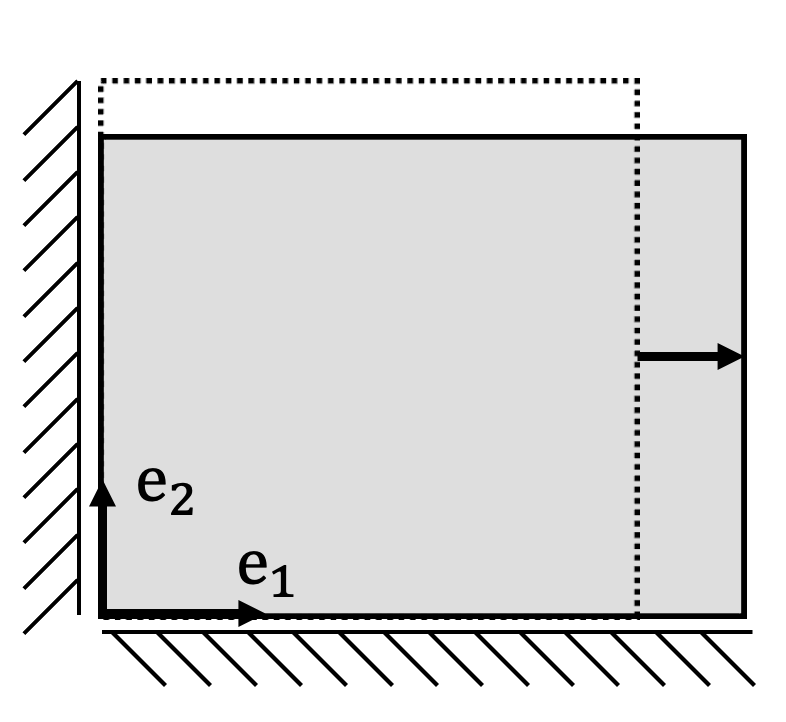
\includegraphics[width=0.5\textwidth]{figures/rectangle.png}
%     \end{center}
    

%     For plane stress without body forces, the momentum balance reduces to
%     \begin{align}
%         (\Lambda + G) \left( \frac{\partial^2 u_1}{\partial x_1^2} + \frac{\partial^2 u_2}{\partial x_1 \partial x_2} \right)
%         + G \left( \frac{\partial^2 u_1}{\partial x_1^2} + 
%             \frac{\partial^2 u_1}{\partial x_2^2} 
%         \right) &= 0 \\
%         (\Lambda + G) \left( \frac{\partial^2 u_1}{\partial x_1 \partial x_2} + \frac{\partial^2 u_2}{\partial x_2^2} \right)
%         + G \left( \frac{\partial^2 u_2}{\partial x_1^2} + 
%             \frac{\partial^2 u_2}{\partial x_2^2}
%         \right) &= 0. 
%     \end{align}
%     We can easily see that all partial derivatives evaluate to zero, hence the momentum balance is fulfilled. In addition, it can be shown easily that the essential boundary conditions are fulfilled. 

%     To prove the natural boundary conditions, we compute the stresses 
%     \begin{align}
%         S_{11} &= 2 G \frac{\partial u_1}{\partial x_1} + \Lambda \left(\frac{\partial u_1}{\partial x_1} + \frac{\partial u_2}{\partial x_2} + \frac{\partial u_3}{\partial x_3} \right)
%         = E \frac{u_0}{l} \\
%         S_{22} &= 2 G \frac{\partial u_2}{\partial x_2} + \Lambda \left(\frac{\partial u_1}{\partial x_1} + \frac{\partial u_2}{\partial x_2} + \frac{\partial u_3}{\partial x_3} \right) 
%         =  0\\
%         S_{12} &= G \left(\frac{\partial u_1}{\partial x_2} + \frac{\partial u_2}{\partial x_1} \right) = 0
%     \end{align}
%     and observe that $S_{12}$ and $S_{22}$ are zero in the entire domain. Hence, both natural boundary conditions are fulfilled as well. The stress $S_{11}$ is proportional to the strain $\frac{u_0}{l}$ with the Young's modulus $E$. This probably matches our expectation, because the stress-free lateral conditions match a tensile test.
% \end{example}


% \begin{example}{Plane strain}{planestrainexample} 
%     If we analyze a structure that is very thick in the 3-direction, there will be no changes of displacement along that direction and we may assume \emph{plane strain}, i.e. $u_3=0$ and $\frac{\partial \bullet}{\partial x_3}=0$. 
    
%     Consider a two-dimensional rectangle $\Omega = [0,l]^2$ which is subjected to the following essential boundary conditions
%     \begin{equation}
%         u_1(0, x_2) = 0     \quad
%         u_1(l, x_2) = u_0   \quad
%         u_2(x_1, 0) = 0
%     \end{equation}
%     and the following natural boundary conditions 
%     \begin{equation}
%         S_{12}(x_1, 0) = 0  \quad
%         S_{12}(x_1, l) = 0  \quad
%         S_{22}(x_1, 0) = 0  \quad
%         S_{22}(x_1, l) = 0.
%     \end{equation}

%     Show that 
%     \begin{equation}
%         u_1 (\mathbf{x}) = u_0 \frac{x_1}{l} \quad
%         u_2 (\mathbf{x}) = - u_0 \frac{\nu}{1-\nu} \frac{x_2}{l}\quad
%         u_3 (\mathbf{x}) = 0
%     \end{equation}
%     solves the isotropic linear elastic problem.

%     \begin{center}
%         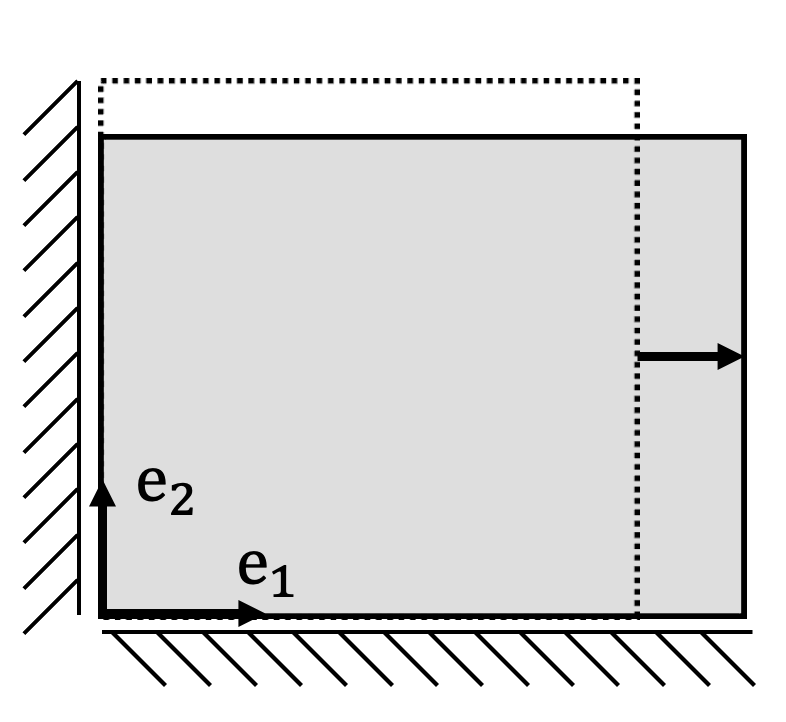
\includegraphics[width=0.5\textwidth]{figures/rectangle.png}
%     \end{center}
    

%     For plane strain and without body forces, the momentum balance reduces to
%     \begin{align}
%         (\Lambda + G) \left( \frac{\partial^2 u_1}{\partial x_1^2} + \frac{\partial^2 u_2}{\partial x_1 \partial x_2} \right)
%         + G \left( \frac{\partial^2 u_1}{\partial x_1^2} + 
%             \frac{\partial^2 u_1}{\partial x_2^2} 
%         \right) &= 0 \\
%         (\Lambda + G) \left( \frac{\partial^2 u_1}{\partial x_1 \partial x_2} + \frac{\partial^2 u_2}{\partial x_2^2} \right)
%         + G \left( \frac{\partial^2 u_2}{\partial x_1^2} + 
%             \frac{\partial^2 u_2}{\partial x_2^2}
%         \right) &= 0. 
%     \end{align}
%     We can easily see that all partial derivatives evaluate to zero, hence the momentum balance is fulfilled. In addition, it can be shown easily that the essential boundary conditions are fulfilled. 

%     To prove the natural boundary conditions, we compute 
%     \begin{align}
%         S_{11} &= 2 G \frac{\partial u_1}{\partial x_1} + \Lambda \left(\frac{\partial u_1}{\partial x_1} + \frac{\partial u_2}{\partial x_2} \right) = \frac{E}{1-\nu^2} \frac{u_0}{l} \\
%         S_{22} &= 2 G \frac{\partial u_2}{\partial x_2} + \Lambda \left(\frac{\partial u_1}{\partial x_1} + \frac{\partial u_2}{\partial x_2} \right) = 0 \\
%         S_{12} &= G \left(\frac{\partial u_1}{\partial x_2} + \frac{\partial u_2}{\partial x_1} \right) = 0
%     \end{align}
%     and observe that both stresses are zero in the entire domain. Hence, both natural boundary conditions are fulfilled as well.
% \end{example}

\section{Weak form}
To solve Equation \eqref{eq:linear_momentum_balance}, which is known as the \emph{strong form} of the linear elastic problem, the displacement field has to be twice differentiable. 
We can relax that requirement by computing the \emph{weak form} of the equation. This is done by contracting the equation with a test function $\mathbf{v} \in \mathcal{H}^1_0 (\Omega) $ and integrating it over the entire domain $\Omega$. Here, the test function is of the same type as $\mathbf{u}$, i.e. it is also a vector function. The space $\mathcal{H}^1_0 (\Omega)$ denotes the \emph{Sobolev space} on $\Omega$, i.e. a function space in which $\mathbf{v}$ becomes zero at the essential boundary and has square integrable derivatives. This is a bit technical, but the steps to get there are straight forward: 
\begin{enumerate}
    \item Contract the equation with test function $\mathbf{v}$
    \item Integrate over domain $\Omega$
    \item Simplify the expressions using the identity 
        \begin{equation}
            (\nabla \cdot \mathbf{S}) \cdot \mathbf{v} = \nabla \cdot (\mathbf{S} \cdot \mathbf{v}) - \mathbf{S} : \nabla \mathbf{v}
            \label{eq:divergence_identity}
        \end{equation}
    and the divergence theorem
    \begin{equation}
        \int_\Omega \nabla \cdot (\bullet) \text{d}V = \int_{\partial \Omega} (\bullet) \cdot \mathbf{n} \text{d}A.
        \label{eq:divergence_theorem}
    \end{equation}
\end{enumerate}

\begin{example}{Using index notation to proof Equation \ref{eq:divergence_identity}}{divergence_identity_example} 
    We can prove Equation \ref{eq:divergence_identity} using index notation and the product rule: 
    \begin{equation}
        \nabla \cdot (\mathbf{S} \cdot \mathbf{v}) = \sum_{i,j} \frac{\partial (S_{ij} v_j)}{\partial x_i} = \sum_{i,j}\frac{\partial S_{ij}}{\partial x_i} v_j + \sum_{i,j} S_{ij} \frac{\partial v_j}{\partial x_i}
    \end{equation}
    Rewriting the right side to symbolic notation yields
    \begin{equation}
        \nabla \cdot (\mathbf{S} \cdot \mathbf{v}) = (\nabla \cdot \mathbf{S}) \cdot \mathbf{v} + \mathbf{S} : \nabla \mathbf{v}.
    \end{equation}
\end{example}

Contracting with the test function and integrating Equation \eqref{eq:linear_momentum_balance} gives
\begin{equation}
    \int_\Omega (\nabla \cdot \mathbf{S}) \cdot \mathbf{v} \text{d}V
    + \int_\Omega \mathbf{b} \cdot \mathbf{v} \text{d}V = 0 \quad \forall \mathbf{v},
    \label{eq:weak_form_raw}
\end{equation}
which is a scalar equation. We can use the identity provided in Equation \eqref{eq:divergence_identity} to expand the first term yielding
\begin{equation}
    \int_\Omega \nabla \cdot (\mathbf{S} \cdot \mathbf{v}) \text{d}V
    - \int_\Omega \mathbf{S} : \nabla \mathbf{v} \text{d}V
    + \int_\Omega \mathbf{b} \cdot \mathbf{v} \text{d}V = 0 \quad \forall \mathbf{v}.
\end{equation}
We can now use the divergence theorem in Equation \eqref{eq:divergence_theorem} to compute 
\begin{equation}
    \int_{\partial \Omega} (\mathbf{S} \cdot \mathbf{v}) \cdot \mathbf{n} \text{d}A
    - \int_\Omega \mathbf{S} : \nabla \mathbf{v} \text{d}V
    + \int_\Omega \mathbf{b} \cdot \mathbf{v} \text{d}V = \mathbf{0} \quad \forall \mathbf{v}.
\end{equation}
Using the fact that $\mathbf{v}$ is zero on the essential boundary, that $\mathbf{S}$ is symmetric and that $\mathbf{S}\cdot \mathbf{n} = \mathbf{t}$ at the natural boundary, we arrive at the simplified weak form of linear elasticity 
\begin{equation}
    \int_{\partial \Omega_N} \mathbf{t} \cdot \mathbf{v} \text{d}A
    - \int_\Omega \mathbf{S} : \nabla \mathbf{v} \text{d}V
    + \int_\Omega \mathbf{b} \cdot \mathbf{v} \text{d}V = 0 \quad \forall \mathbf{v}.
\end{equation}
Using the symmetry of $\mathbf{S}$ and replacing the material model, we may denote this in the commonly found form
\begin{equation}
    \int_{\partial \Omega_N} \mathbf{t} \cdot \mathbf{v} \text{d}A
    - \int_\Omega \mathbf{E}(\mathbf{u}) : \mathbb{C} :  \mathbf{E}(\mathbf{v}) \text{d}V
    + \int_\Omega \mathbf{b} \cdot \mathbf{v} \text{d}V = 0 \quad \forall \mathbf{v}.
\end{equation}
It can be proven that this is equivalent to the strong form as long as we require the equation to hold for arbitrary $\mathbf{v}$. We may interpret this formulation as being similar to the principal of virtual work with the test function taking the role of a virtual displacement.
The benefit of this formulation is that the solution $\mathbf{u}$ has to be only differentiable once, because we got rid of the divergence operator in front of $\mathbf{S}$.

\section{Spatial discretization in 2D}
We can only solve the linear elastic problem analytically on simple geometries and with some assumptions. In general, on real world complex domains $\Omega$, we cannot solve it analytically. However, we can divide the problem in many small sub-problems on simple geometries and try to find a combined solution of these.

The core idea of finite elements is the discretization of a continuous domain $\Omega \subset \mathcal{R}^3$ into a finite number of $M$ small elements $\Omega_j$. Then, the weak form can be expressed as 
\begin{equation}
    \sum_{j=0}^{M-1} \int_{\partial \Omega_{N,j}} \mathbf{t} \cdot \mathbf{v} \text{d}A
    - \sum_{j=0}^{M-1} \int_{\Omega_j} \mathbf{E}(\mathbf{u}) : \mathbb{C} :  \mathbf{E}(\mathbf{v}) \text{d}V
    + \sum_{j=0}^{M-1} \int_{\Omega_j} \mathbf{b} \cdot \mathbf{v} \text{d}V = 0 \quad \forall \mathbf{v}.
    \label{eq:discretized_weak_form_3d}
\end{equation}

If we reduce the problem to a two dimensional domain, i.e. $\Omega \subset \mathcal{R}^2$ we can simplify this to  
\begin{equation}
    \sum_{j=0}^{M-1} 
    \underbrace{\int_{\partial \Omega_{N,j}} \mathbf{t} \cdot \mathbf{v} \text{d}s}_\textrm{Boundary traction}
    - \sum_{j=0}^{M-1} d_j  
    \underbrace{\int_{\Omega_j} \mathbf{E}(\mathbf{u}) : \mathbb{C} :  \mathbf{E}(\mathbf{v}) \text{d}A}_\textrm{Strain energy}
    + \sum_{j=0}^{M-1} \underbrace{\int_{\Omega_j} \mathbf{b} \cdot \mathbf{v} \text{d}A}_\textrm{Body forces} = 0 \quad \forall \mathbf{v}.
    \label{eq:discretized_weak_form}
\end{equation}
with the constant thickness of each element $d_j$, a traction $\mathbf{t}$ describing force per length and a body force $\mathbf{b}$ describing force per unit area.

Within each element $\Omega_j$, we can approximate the solution with so-called \emph{shape functions}. These are simple linear or quadratic functions that are continuous across element edges and we define them on a \emph{reference element}. In a two-dimensional problem, this reference element typically has as triangular or quadrilateral shape and in a three-dimensional problem, this reference element typically has a tetrahedral or hexahedral shape. We focus on two-dimensional linear quadrilateral elements in this lecture, but equivalent formulations can be found for any element type. 

\begin{example}{Linear quadrilateral elements}{quadshapeexample} 
    First of all, we describe the reference element in its own local coordinate system with coordinates $\xi_1$ and $\xi_2$. Later, we can transfer it to any other shape and position by scaling and shifting the element to global coordinates. 

    \begin{center}
        \includesvg[width=0.5\textwidth]{figures/reference_element.svg}
    \end{center}

    In this local coordinate system, we can interpolate any variable defined on nodes $\mathbf{a}_j$ by an approximation
    \begin{equation}
        a = \mathbf{N}(\pmb{\xi}) \cdot  \mathbf{a}_j
    \end{equation}
    with shape functions $\mathbf{N}(\pmb{\xi})$ interpolating the values at the four element nodes
    \begin{equation}
        \mathbf{a}_j = 
        \begin{pmatrix}
            a_j^0\\ 
            a_j^1\\ 
            a_j^2\\ 
            a_j^3\\
        \end{pmatrix}.
    \end{equation}
    For a quadrilateral linear reference element, the shape functions are given by 
    \begin{equation}
        \mathbf{N}(\pmb{\xi}) = \frac{1}{4}
        \begin{pmatrix}
            (1-\xi_1)(1-\xi_2) \\
            (1+\xi_1)(1-\xi_2) \\
            (1+\xi_1)(1+\xi_2) \\
            (1-\xi_1)(1+\xi_2)
        \end{pmatrix}
    \end{equation}
    such that each function assumes the value 1 at one node of the element and the value 0 at all other nodes of the element. The four shape functions $N_1, N_2, N_3, N_4$ of the linear quadrilateral reference element are displayed in the following figure for $\Omega_j = [-1,1]^2$.
    

    \begin{center}
        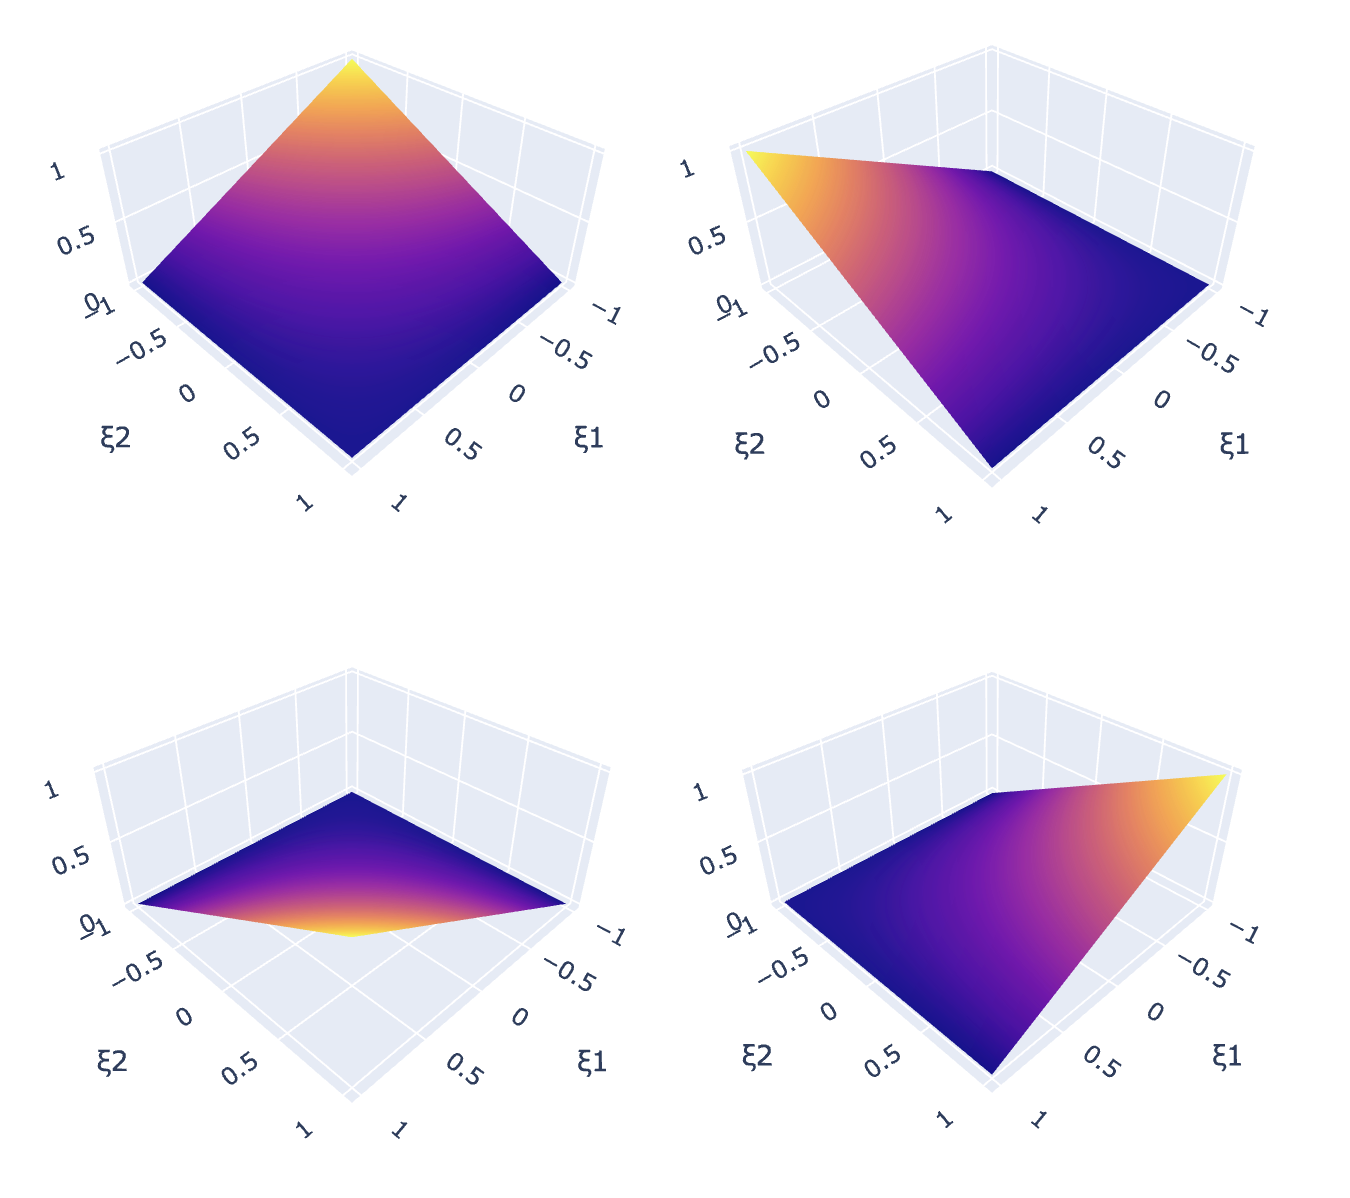
\includegraphics[width=0.7\textwidth]{figures/quad_shape_functions.png}
    \end{center}

    The shape functions enable us to compute gradients on each reference element as 
    \begin{equation}
        \nabla_\xi a = \mathbf{B}_\textrm{ref}(\pmb{\xi}) \cdot  \mathbf{a}_j
    \end{equation}
    with 
    \begin{equation}
        \mathbf{B}^\textrm{ref}(\pmb{\xi})
        =  \nabla_\xi \mathbf{N}(\pmb{\xi}) 
        = 
        \begin{pmatrix}
            \frac{\partial \mathbf{N}(\pmb{\xi})}{\partial \xi_1} \\ 
            \frac{\partial \mathbf{N}(\pmb{\xi})}{\partial \xi_2} 
        \end{pmatrix} 
        = \frac{1}{4}
        \begin{pmatrix}
            -1 + \xi_2 & 1 - \xi_2 & 1 + \xi_2 & -1 - \xi_2 \\
            -1 + \xi_1 & -1 - \xi_1 & 1 + \xi_1 & 1 - \xi_1
        \end{pmatrix}
    \end{equation}

    These gradients are formulated w.r.t. the reference system $\xi_1, \xi_2$. Employing the chain rule, we may formulate gradients w.r.t. to the global coordinates as 
    \begin{equation}
        \nabla a = 
        \underbrace{
        \begin{pmatrix}
            \frac{\partial \xi_1}{\partial x_1} & \frac{\partial \xi_2}{\partial x_1} \\
            \frac{\partial \xi_1}{\partial x_2} & \frac{\partial \xi_2}{\partial x_2} \\
        \end{pmatrix}
        }_\textrm{Chain rule}
        \cdot 
        \mathbf{B}^\textrm{ref}(\pmb{\xi}) \cdot  \mathbf{a}_j
    \end{equation}

    We may use the shape functions $\mathbf{N}(\pmb{\xi})$ to interpolate the nodal positions of an element $j$ by 
    \begin{equation}
        x_1(\pmb{\xi})
        = 
        \mathbf{N}(\pmb{\xi})
        \cdot 
        \begin{pmatrix}
            {(x_1)}_j^0 \\
            {(x_1)}_j^1 \\
            {(x_1)}_j^2 \\
            {(x_1)}_j^3 \\
        \end{pmatrix}
        , \quad
        x_2(\pmb{\xi})
        = 
        \mathbf{N}(\pmb{\xi})
        \cdot 
        \begin{pmatrix}
            {(x_2)}_j^0 \\
            {(x_2)}_j^1 \\
            {(x_2)}_j^2 \\
            {(x_2)}_j^3 \\
        \end{pmatrix}
    \end{equation}
    or use $\mathbf{B}^\textrm{ref}(\pmb{\xi})$ to compute the gradients
    \begin{equation}
        \begin{pmatrix}
            \frac{\partial x_1}{\partial \xi_1} \\
            \frac{\partial x_1}{\partial \xi_2}\\
        \end{pmatrix}
        = 
        \mathbf{B}^\textrm{ref}(\pmb{\xi})
        \cdot 
        \begin{pmatrix}
            {(x_1)}_j^0 \\
            {(x_1)}_j^1 \\
            {(x_1)}_j^2 \\
            {(x_1)}_j^3 \\
        \end{pmatrix}
        , \quad
        \begin{pmatrix}
            \frac{\partial x_2}{\partial \xi_1} \\
            \frac{\partial x_2}{\partial \xi_2}\\
        \end{pmatrix}
        = 
        \mathbf{B}^\textrm{ref}(\pmb{\xi})
        \cdot 
        \begin{pmatrix}
            {(x_2)}_j^0 \\
            {(x_2)}_j^1 \\
            {(x_2)}_j^2 \\
            {(x_2)}_j^3 \\
        \end{pmatrix}.
    \end{equation}
    The latter gradients can be used to compute the \emph{Jacobian} 
    \begin{equation}
        \mathbf{J}_j(\pmb{\xi})
        = 
        \begin{pmatrix}
            \frac{\partial x_1}{\partial \xi_1} & \frac{\partial x_2}{\partial \xi_1} \\
            \frac{\partial x_1}{\partial \xi_2} & \frac{\partial x_2}{\partial \xi_2}
        \end{pmatrix},
    \end{equation}
    which is just the inverse of the missing term of the chain rule. Hence we can determine the interpolated gradient of $a$ w.r.t. the global coordinate system as 
    \begin{equation}
        \nabla a = 
        \underbrace{
            \mathbf{J}_j^{-1}(\pmb{\xi}) 
            \cdot 
            \mathbf{B}^\textrm{ref}(\pmb{\xi})
            }_{\mathbf{B}(\pmb{\xi})}
        \cdot  \mathbf{a}_j
    \end{equation}
\end{example}

\begin{example}{Gauss–Legendre quadrature}{quadratureexample} 
    In addition to the interpolation, we need to find numerical solutions to the integral. Hence, this is a quick recap of the Gauss-legendre quadrature. 
    
    Consider an integral in $\mathcal{R}$
    \begin{equation}
        \int_{a}^{b} f(x) dx.
    \end{equation}
    We can solve this by transforming it to a unit domain
    \begin{equation}
        \int_{-1}^{1} f(\xi) \frac{\text{d}x}{\text{d}\xi} \text{d}\xi
    \end{equation}
    with 
    \begin{equation}
        \frac{dx}{d\xi} = \frac{b-a}{2}.
    \end{equation}
    For this unit domain, we can express the integral as a summation with tabulated positions $\xi^k$ and weights $w^k$ like
    \begin{equation}
        \int_{-1}^{1} f(\xi) \frac{\text{d}x}{\text{d}\xi} \text{d}\xi
        = \sum_{k=1}^m w^k f(\xi^k) \frac{\text{d}x}{\text{d}\xi} \xi.
    \end{equation}
    This summation via Gauss quadrature is able to integrate polynomials up to an order $2m-1$ exactly. For example, using two points ($m=2$) with 
    \begin{equation}
        \xi^1 = -\frac{1}{\sqrt{3}}, \quad \xi^2 = \frac{1}{\sqrt{3}}
    \end{equation}
    and weights $w^1=1$ and $w^2=1$ enables exact integration of polynomials up to order 3, which is sufficient for our integrals as we approximate the integral functions with linear shape functions. 

    \begin{center}
        \includesvg[width=\textwidth]{figures/gauss_legendre.svg}
    \end{center}
    
    This one-dimensional example can be extended canonically to higher dimensions by replacing $\frac{\text{d}x}{\text{d}\xi}$ with the determinant of the Jacobian and by using positions 
    \begin{equation}
        \pmb{\xi}^1 = \begin{pmatrix}-\frac{1}{\sqrt{3}} \\ -\frac{1}{\sqrt{3}}\end{pmatrix} 
        \quad
        \pmb{\xi}^2 = \begin{pmatrix}-\frac{1}{\sqrt{3}} \\ \frac{1}{\sqrt{3}}\end{pmatrix} 
        \quad
        \pmb{\xi}^3 = \begin{pmatrix}\frac{1}{\sqrt{3}} \\ -\frac{1}{\sqrt{3}}\end{pmatrix} 
        \quad
        \pmb{\xi}^4 = \begin{pmatrix}\frac{1}{\sqrt{3}} \\ \frac{1}{\sqrt{3}}\end{pmatrix} 
        \label{eq:gaussian_weights}
    \end{equation}
    which are indicated as gray points in the sketch of the reference element in the previous example.
\end{example}

In conclusion, the definition of shape functions on an element allows us to interpolate nodal properties (like position, displacements or temperatures) and to compute gradients of these properties within the element. In addition, Gauss-Legendre quadrature allows us to integrate these properties over the element domain and thus to evaluate the integrals in Equation \eqref{eq:discretized_weak_form}. The following subsection addresses this procedure for each of the terms in Equation \eqref{eq:discretized_weak_form}.

\subsection{External work by body forces}
Let's start with the body force term and transform the integral from the original domain to the reference element as
\begin{equation}
    \int_{\Omega_j} \mathbf{b} \cdot \mathbf{v} \text{d}A
    = 
    \int_{\Omega_j^\textrm{ref}} \mathbf{b} \cdot \mathbf{v}(\pmb{\xi})
    \hspace{0.25em} \text{det}\left(\mathbf{J}_j(\pmb{\xi})\right)\text{d}A^\textrm{ref}
\end{equation}
using the determinant of the Jacobian as a scaling factor between $\text{d}A$ and $\text{d}A^\textrm{ref}$. This scaling is equivalent to the usage of $\frac{\text{d}x}{\text{d}\xi}$ in the one-dimensional example. 

We can then use Gauss–Legendre quadrature with two positions per dimension to perform a numerical integration of this term as
\begin{equation}
    \int_{\Omega_j^\textrm{ref}} \mathbf{b} \cdot \mathbf{v}(\pmb{\xi}) \hspace{0.25em}\text{det}\left(\mathbf{J}_j(\pmb{\xi})\right)\text{d}A^\textrm{ref}
    = \sum_{k=1}^4 w^k \text{det}\left(\mathbf{J}_j(\pmb{\xi}^k)\right) \mathbf{b} \cdot \mathbf{v}(\pmb{\xi}^k).
\end{equation}
Essentially, this turns the integral into a weighted sum of function values at specific positions $\pmb{\xi}^k$. In this case, we chose $w^k=1$ and positions according to Equation \eqref{eq:gaussian_weights}.
Using the shape functions, we may then express the last variable using the nodal values of the trial function $\mathbf{v}_j$ as  
\setlength\arraycolsep{-2pt}
\begin{equation}
    \mathbf{v}(\pmb{\xi}^k) 
    =
    \begin{pmatrix}
            N_1(\pmb{\xi}^k) & 0 & N_2(\pmb{\xi}^k) & 0 & N_3(\pmb{\xi}^k) & 0 & N_4(\pmb{\xi}^k) & 0\\
            0 & N_1(\pmb{\xi}^k) & 0 & N_2(\pmb{\xi}^k) & 0 & N_3(\pmb{\xi}^k) & 0 & N_4(\pmb{\xi})\\
    \end{pmatrix}
    \cdot 
    \begin{pmatrix}
            {(v_1)}_j^0 \\
            {(v_2)}_j^0 \\
            {(v_1)}_j^1 \\
            {(v_2)}_j^1 \\
            {(v_1)}_j^2 \\
            {(v_2)}_j^2 \\
            {(v_1)}_j^3 \\
            {(v_2)}_j^3 
    \end{pmatrix}.
    \label{eq:shape_interpolation}
\end{equation}
\setlength\arraycolsep{5pt}
In summary, we transformed the body force term of a single element from 
\begin{equation}
    \int_{\Omega_j} \mathbf{b} \cdot \mathbf{v} \text{d}A  
\end{equation}
to a scalar vector product 
\setlength\arraycolsep{-5pt}
\begin{equation}
    \underbrace{\sum_k \text{det}\left(\mathbf{J}_j(\pmb{\xi}^k)\right) \mathbf{b} \cdot
    \begin{pmatrix}
            N_1(\pmb{\xi}^k) & 0 & N_2(\pmb{\xi}^k) & 0 & N_3(\pmb{\xi}^k) & 0 & N_4(\pmb{\xi}^k) & 0\\
            0 & N_1(\pmb{\xi}^k) & 0 & N_2(\pmb{\xi}^k) & 0 & N_3(\pmb{\xi}^k) & 0 & N_4(\pmb{\xi})\\
    \end{pmatrix}}_{\mathbf{f}^\Omega_j}
    \cdot 
    \mathbf{v}_j
\end{equation}
\setlength\arraycolsep{5pt}
where $\mathbf{f}^\Omega_j \in \mathcal{R}^8$ describes the nodal body forces on element $j$. 

\subsection{Strain energy term}
Similar to the body force term, we can evaluate the strain energy term of an element in Equation \eqref{eq:discretized_weak_form} by transforming the integral and applying Gauss-Legendre quadrature as 
\begin{equation}
    \int_{\Omega_j} \mathbf{E}(\mathbf{u}) : \mathbb{C} :  \mathbf{E}(\mathbf{v}) \text{d}A 
    = \sum_k \mathbf{E}\left(\mathbf{u}(\pmb{\xi^k})\right) : \mathbb{C} :  \mathbf{E}\left(\mathbf{v}(\pmb{\xi^k})\right)  \text{det}\left(\mathbf{J}_j(\pmb{\xi}^k)\right).
\end{equation}
The double contraction is unnecessarily complex for a two-dimensional problem and we can simplify it as follows:
\begin{equation}
    \mathbf{E}\left(\mathbf{u}(\pmb{\xi^k})\right) : \mathbb{C} :  \mathbf{E}\left(\mathbf{v}(\pmb{\xi^k})\right) = 
    \pmb{\varepsilon}\left(\mathbf{u}(\pmb{\xi}^k)\right)
    \cdot 
    \mathbf{C}
    \cdot 
    \pmb{\varepsilon}\left(\mathbf{v}(\pmb{\xi}^k)\right)
\end{equation}
with a two-dimensional stiffness matrix
\begin{align}
        \mathbf{C} &= \begin{pmatrix}
        2G+\Lambda & \Lambda & 0 \\
        \Lambda & 2G+\Lambda &  0 \\
        0 & 0 & G \\
    \end{pmatrix} \textrm{(isotropic plane strain)}\\
    \mathbf{C} &= \frac{E}{1-\nu^2}\begin{pmatrix}
        1 & \nu & 0 \\
        \nu & 1 &  0 \\
        0 & 0 & (1-\nu)/2 \\
    \end{pmatrix} \textrm{(isotropic plane stress)}
\end{align}
and with two-dimensional strains
\begin{equation}
    \pmb{\varepsilon}(\mathbf{u}) = 
    \begin{pmatrix}
        \frac{\partial u_1}{\partial x_1} \\ 
        \frac{\partial u_2}{\partial x_2} \\
        \frac{\partial u_1}{\partial x_2} + \frac{\partial u_2}{\partial x_1}\\
    \end{pmatrix}
    \quad 
    \textrm{and}
    \quad
    \pmb{\varepsilon}(\mathbf{v}) = 
    \begin{pmatrix}
        \frac{\partial v_1}{\partial x_1} \\ 
        \frac{\partial v_2}{\partial x_2} \\
        \frac{\partial v_1}{\partial x_2} + \frac{\partial v_2}{\partial x_1}\\
    \end{pmatrix}.
\end{equation}
We can express the strain terms with shape functions as 
\setlength\arraycolsep{2pt}
\begin{equation}
    \pmb{\varepsilon}\left(\mathbf{v}\right)
    =
    \underbrace{
    \begin{pmatrix}
            B_{11}(\pmb{\xi}^k) & 0 & B_{12}(\pmb{\xi}^k) & 0 & B_{13}(\pmb{\xi}^k) & 0 & B_{14}(\pmb{\xi}^k) & 0\\
            0 & B_{21}(\pmb{\xi}^k) & 0 & B_{22}(\pmb{\xi}^k) & 0 & B_{23}(\pmb{\xi}^k) & 0 & B_{24}(\pmb{\xi}^k)\\
            B_{21}(\pmb{\xi}^k) & B_{11}(\pmb{\xi}^k) & B_{22}(\pmb{\xi}^k) & B_{12}(\pmb{\xi}^k) & B_{23}(\pmb{\xi}^k) & B_{13}(\pmb{\xi}^k) & B_{24}(\pmb{\xi}^k) & B_{14}(\pmb{\xi}^k)\\
    \end{pmatrix} 
    }_{\mathbf{D}}
    \cdot 
    \mathbf{v}_j
\end{equation}
\setlength\arraycolsep{5pt}
for the derivatives of the trial function and analogous for the displacements. In conclusion, we can transform the integral 
\begin{equation}
    d_j \int_{\Omega_j} \mathbf{E}(\mathbf{u}) : \mathbb{C} :  \mathbf{E}(\mathbf{v}) \text{d}A 
\end{equation}
to a matrix vector product 
\begin{equation}
    \mathbf{u}_j \cdot 
    \underbrace{
    d_j 
    \underbrace{ 
    \sum_k \text{det}\left(\mathbf{J}_j(\pmb{\xi}^k)\right)\mathbf{D}^\top \cdot \mathbf{C} \cdot \mathbf{D}}_{\mathbf{k}^0_j}
    }_{\mathbf{k}_j}
    \cdot \mathbf{v}_j
\end{equation}
with an element stiffness matrix $\mathbf{k}_j = d_j  \mathbf{k}^0_j \in \mathcal{R}^{8x8}$. 

\subsection{External work by boundary traction}
Finally, the boundary traction term in Equation \eqref{eq:discretized_weak_form} is treated in a similar fashion to the previous terms. However, the boundary of a two-dimensional domain is just a line and we integrate it with two points along the element edge as 
\begin{equation}
    \int_{\partial \Omega_{N,j}} \mathbf{t} \cdot \mathbf{v} \text{d}s
    =
    \sum_k \mathbf{t}(\xi^k) \cdot \mathbf{v}(\xi^k) \frac{\partial x}{\partial \xi} 
\end{equation}

Using Equation \eqref{eq:shape_interpolation}, we may denote this as 
\setlength\arraycolsep{-5pt}
\begin{equation}
    \underbrace{\sum_k \frac{\partial x}{\partial \xi} \mathbf{t}(\pmb{\xi}^k) \cdot
    \begin{pmatrix}
            N_1(\pmb{\xi}^k) & 0 & N_2(\pmb{\xi}^k) & 0 & N_3(\pmb{\xi}^k) & 0 & N_4(\pmb{\xi}^k) & 0\\
            0 & N_1(\pmb{\xi}^k) & 0 & N_2(\pmb{\xi}^k) & 0 & N_3(\pmb{\xi}^k) & 0 & N_4(\pmb{\xi})\\
    \end{pmatrix}}_{\mathbf{f}^\Gamma_j}
    \cdot 
    \mathbf{v}_j
\end{equation}
\setlength\arraycolsep{5pt}
where $\mathbf{f}^\Gamma_j \in \mathcal{R}^8$ describes the nodal traction forces on element $j$. 

\section{Assembly of linear systems of equations}

At this point, we can transform Equation \eqref{eq:discretized_weak_form} to 
\begin{equation}
    \sum_{j=0}^{M-1} \mathbf{f}^\Gamma_j \cdot \mathbf{v}_j
    - \sum_{j=0}^{M-1} \mathbf{u}_j \cdot \mathbf{k}_j \cdot \mathbf{v}_j
    + \sum_{j=0}^{M-1} \mathbf{f}^\Omega_j \cdot \mathbf{v}_j = 0 \quad \forall \mathbf{v}_j.
\end{equation}
with element-wise matrices that are very similar to the truss system from Chapter 5. Rearranging this equation yields 
\begin{equation}
    \sum_{j=0}^{M-1} \mathbf{v}_j \cdot \left( \mathbf{f}^\Gamma_j + \mathbf{f}^\Omega_j \right)
    = \sum_{j=0}^{M-1} \mathbf{v}_j \cdot \mathbf{k}_j \cdot \mathbf{u}_j \quad \forall \mathbf{v}_j.
\end{equation}
We can assemble this sum of linear equation systems to a global equation system 
\begin{equation}
    \mathbf{v} \cdot \mathbf{f} = \mathbf{v} \cdot \mathbf{K} \cdot \mathbf{u}
\end{equation}
with 
\begin{equation}
    \mathbf{v} = 
    \begin{pmatrix}
    \begin{smallmatrix}
        \dots \\ (v_1)^0_j \\ (v_2)^0_j \\ \dots \\ (v_1)^1_j \\ (v_2)^1_j \\ \dots \\ (v_1)^2_j \\ (v_2)^2_j \\ \dots \\ (v_1)^3_j \\ (v_2)^3_j \\ \dots \\
    \end{smallmatrix}
    \end{pmatrix}
    \quad
    \text{and}
    \quad
    \mathbf{u}
    \begin{pmatrix}
    \begin{smallmatrix}
        \dots \\ (u_1)^0_j \\ (u_2)^0_j \\ \dots \\ (u_1)^1_j \\ (u_2)^1_j \\ \dots \\
        \dots \\ (u_1)^2_j \\ (u_2)^2_j \\ \dots \\ (u_1)^3_j \\ (u_2)^3_j \\ \dots
    \end{smallmatrix}
    \end{pmatrix}
    \quad
    \text{and}
    \quad
    \mathbf{f} = 
    \sum_j
    \begin{pmatrix}
    \begin{smallmatrix}
        \dots \\ (f^\Gamma_1)^0_j + (f^\Omega_1)^0_j \\ (f^\Gamma_2)^0_j + (f^\Omega_2)^0_j \\ \dots \\ (f^\Gamma_1)^1_j + (f^\Omega_1)^1_j \\ (f^\Gamma_2)^1_j + (f^\Omega_2)^1_j\\ \dots \\ (f^\Gamma_1)^2_j + (f^\Omega_1)^2_j \\ (f^\Gamma_2)^2_j + (f^\Omega_2)^2_j \\ \dots \\ (f^\Gamma_1)^3_j + (f^\Omega_1)^3_j \\ (f^\Gamma_2)^3_j + (f^\Omega_2)^3_j \\ \dots \\
    \end{smallmatrix}
    \end{pmatrix}.
\end{equation}
and
\begin{equation}
    \mathbf{K} =
    \sum_j
    \underbrace{
    \begin{pmatrix}
    \begin{smallmatrix}
    \dots & \dots & \dots & \dots & \dots & \dots & \dots & \dots & \dots & \dots & \dots & \dots & \dots \\
    \dots & (k_{11})_j & (k_{12})_j & \dots & (k_{13})_j & (k_{14})_j & \dots & (k_{15})_j & (k_{16})_j & \dots & (k_{17})_j & (k_{18})_j & \dots  \\
     \dots & (k_{21})_j & (k_{22})_j & \dots & (k_{23})_j & (k_{24})_j & \dots & (k_{25})_j & (k_{26})_j & \dots & (k_{27})_j & (k_{28})_j & \dots  \\
    \dots & \dots & \dots & \dots & \dots & \dots & \dots  \\
    \dots & (k_{31})_j & (k_{32})_j & \dots & (k_{33})_j & (k_{34})_j & \dots & (k_{35})_j & (k_{36})_j & \dots & (k_{37})_j & (k_{38})_j & \dots  \\
    \dots & (k_{41})_j & (k_{42})_j & \dots & (k_{43})_j & (k_{44})_j & \dots & (k_{45})_j & (k_{46})_j & \dots & (k_{47})_j & (k_{48})_j & \dots  \\
    \dots & \dots & \dots & \dots & \dots & \dots & \dots  \\
    \dots & (k_{51})_j & (k_{52})_j & \dots & (k_{53})_j & (k_{54})_j & \dots & (k_{55})_j & (k_{56})_j & \dots & (k_{57})_j & (k_{58})_j & \dots  \\
     \dots & (k_{61})_j & (k_{62})_j & \dots & (k_{63})_j & (k_{64})_j & \dots & (k_{65})_j & (k_{66})_j & \dots & (k_{67})_j & (k_{68})_j & \dots  \\
    \dots & \dots & \dots & \dots & \dots & \dots & \dots  \\
    \dots & (k_{71})_j & (k_{72})_j & \dots & (k_{73})_j & (k_{74})_j & \dots & (k_{75})_j & (k_{76})_j & \dots & (k_{77})_j & (k_{78})_j & \dots  \\
    \dots & (k_{81})_j & (k_{82})_j & \dots & (k_{83})_j & (k_{84})_j & \dots & (k_{85})_j & (k_{86})_j & \dots & (k_{87})_j & (k_{88})_j & \dots  \\
    \dots & \dots & \dots & \dots & \dots & \dots & \dots  \\
    \end{smallmatrix}
    \end{pmatrix}
    }_{\mathbf{K}_j}
\end{equation}
where the 64 entries of the element stiffness are placed at corresponding positions for the global degrees of freedom in a global stiffness tensor $\mathbf{K}$. Assuming $\mathbf{u}_0=\mathbf{0}$ and using the fact that the test function $\mathbf{v}$ is arbitrary (but zero on the essential boundary) we end up with a reduced system 
\begin{equation}
     \mathbf{f}_\textrm{red} = \mathbf{K}_\textrm{red} \cdot \mathbf{u}_\textrm{red} 
     \label{eq:reduced_system_fem}
\end{equation}
just like previously with the truss system in Chapter 5. Now it comes down to solving this linear system of equations in order to compute the solution $\mathbf{u}_\textrm{red}$.

\begin{example}{Finite element solution of a cantilever beam}{femexample} 
    The following example shows a simple 2D cantilever beam discretized with 722 nodes and 666 linear quad elements. This results in 1444 degrees of freedom in total. The cantilever beam is subjected to a point load at the tip and clamped at one side. There is no body force acting on it ($\mathbf{b} = \mathbf{0}$).
    \begin{center}
        \includesvg[width=0.8\textwidth]{figures/cantilever_fem.svg}
    \end{center}
    Evaluation of the integrals and assembling it leads to a global system 
    \begin{equation}
        \mathbf{f} = \mathbf{K} \mathbf{u}
    \end{equation}
    with $\mathbf{f}, \mathbf{u} \in \mathcal{R}^{1444}$ and $\mathbf{K} \in \mathcal{R}^{1444x1444}$. Elimination of the 38 constrained degrees of freedom results in 
    \begin{equation}
        \mathbf{f}_\textrm{red} = \mathbf{K}_\textrm{red} \mathbf{u}_\textrm{red}
    \end{equation}
    with $\mathbf{f}_\textrm{red}, \mathbf{u}_\textrm{red} \in \mathcal{R}^{1406}$ and $\mathbf{K}_\textrm{red} \in \mathcal{R}^{1406x1406}$. This can be solved for $\mathbf{u}_\textrm{red}$ representing the displacements at each node. The subsequent figure shows the norm of the displacement interpolated with linear shape functions.
    \begin{center}
        \includesvg[width=0.8\textwidth]{figures/cantilever_fem_solved.svg}
    \end{center}
\end{example}

\bibliographystyle{unsrtnat}
\bibliography{literature} 



